%%%%%%%%%%%%%%%%%%%%%%%%%%%%%%%%%%%%%%%%%
% Stylish Article
% LaTeX Template
% Version 2.2 (2020-10-22)
%
% This template has been downloaded from:
% http://www.LaTeXTemplates.com
%
% Original author:
% Mathias Legrand (legrand.mathias@gmail.com) 
% With extensive modifications by:
% Vel (vel@latextemplates.com)
%
% License:
% CC BY-NC-SA 3.0 (http://creativecommons.org/licenses/by-nc-sa/3.0/)
%
%%%%%%%%%%%%%%%%%%%%%%%%%%%%%%%%%%%%%%%%%

%----------------------------------------------------------------------------------------
%	PACKAGES AND OTHER DOCUMENT CONFIGURATIONS
%----------------------------------------------------------------------------------------

\documentclass[fleqn,10pt]{SelfArx} % Document font size and equations flushed left

\usepackage[english]{babel} % Specify a different language here - english by default

\usepackage{lipsum} % Required to insert dummy text. To be removed otherwise

%----------------------------------------------------------------------------------------
%	COLUMNS
%----------------------------------------------------------------------------------------

\setlength{\columnsep}{0.55cm} % Distance between the two columns of text
\setlength{\fboxrule}{0.75pt} % Width of the border around the abstract

%----------------------------------------------------------------------------------------
%	COLORS
%----------------------------------------------------------------------------------------

\definecolor{color1}{RGB}{0,0,90} % Color of the article title and sections
\definecolor{color2}{RGB}{0,20,20} % Color of the boxes behind the abstract and headings

%----------------------------------------------------------------------------------------
%	HYPERLINKS
%----------------------------------------------------------------------------------------

\usepackage{hyperref} % Required for hyperlinks

\hypersetup{
	hidelinks,
	colorlinks,
	breaklinks=true,
	urlcolor=color2,
	citecolor=color1,
	linkcolor=color1,
	bookmarksopen=false,
	pdftitle={Title},
	pdfauthor={Author},
}

%----------------------------------------------------------------------------------------
%	ARTICLE INFORMATION
%----------------------------------------------------------------------------------------

\JournalInfo{Machine Learning for Natural Language Processing 1} % Journal information
\Archive{Fall Semester 2022} % Additional notes (e.g. copyright, DOI, review/research article)

\PaperTitle{Latent Dirichlet Allocation VS. Combined Topic Modeling: Are New Approaches to Topic Modeling Really Outperforming Traditional Ones?} % Article title


\Keywords{Latent Dirichlet Allocation --- Combined Topic Models --- Unsupervised Learning --- NLP} % Keywords - if you don't want any simply remove all the text between the curly brackets
\newcommand{\keywordname}{Keywords} % Defines the keywords heading name

%----------------------------------------------------------------------------------------
%	ABSTRACT
%----------------------------------------------------------------------------------------

\Abstract{Topic modeling is a statistical technique for discovering the latent topics underlying a collection of documents. This paper presents a comparison of two topic modeling algorithms, Latent Dirichlet Allocation (LDA) and Combined Topic Models (CTM). We find that on the DBLP Database, a large database containing metadata on computer science (and related) publications, CTM and LDA approximately perform equivalent when measuring coherence with human intuition.}

%----------------------------------------------------------------------------------------

\begin{document}

\maketitle % Output the title and abstract box

\tableofcontents % Output the contents section

\thispagestyle{empty} % Removes page numbering from the first page

%----------------------------------------------------------------------------------------
%	ARTICLE CONTENTS
%----------------------------------------------------------------------------------------

\section*{Introduction} % The \section*{} command stops section numbering
Topic modeling is a type of statistical modeling for discovering the abstract "topics" that occur in a collection of documents. Topic modeling is a powerful tool for improving information retrieval, document classification, topic discovery, and even machine translation. The most well known technique for topic modeling in Natural Langugage Processing (NLP) is LDA. LDA is a topic modeling algorithm that is particularly well-suited for discovering hidden, latent themes within a set of documents. It can be thought of as a dimensionality reduction technique that is able to find structure in high-dimensional space. LDA is an unsupervised learning algorithm, which means that it does not require any training data. Instead, LDA uses a statistical approach to learn about the hidden structure of the documents in a collection. As such, LDA is of probabilistic nature, which means that it is based on a statistical model of the joint distribution of words and topics in a document. The output of LDA is a set of topics, each of which is represented by a set of words.

As LDA frequently results in word groups that are not coherent, which makes them hard to interpret, new, more advanced techniques have been proposed. One approach is the CTM from Bianchi et al. 2021. It is a neural topic model making use of contextual embeddings.They promise that their "approach produces more meaningful and coherent topics than traditional bag-of-words topic models and recent neural models".

\section{Methods}

\subsection{Preprocessing}
Preprocessing is an essential step in any data analysis workflow. It is usually the first step in the process, and it can have a significant impact on the results of downstream tasks.

In order to get better performance from our topic models, we applied the following preprocessing:

\begin{enumerate}[noitemsep]
    \item Lowercasing
    \item Lemmatization
    \item Removing stopwords
    \item Remove punctuation
\end{enumerate}


Lemmatization is a process of converting a word to its base form. This can be useful for downstream tasks such as topic modeling, when grouping together different inflected forms of the same word. Further, common words that are not informative, such as “the”, “is”, and “are” (stopwords) are filtered out. Removing punctuation is also a common preprocessing step, especially when working with text data. This can help to simplify the data and make it more uniform. We also lowercased the data as we believe that grammatical idiosyncrasies should not be considered for topic modeling and might lead to biased results when not handled.

\subsection{Project Outline and Data}

In this paper we want to outline the comparison between LDA and CTM. For that we compare the results of both methods with 5 topics
(the number of topics to be modeled is a hyper parameter of any topics model). We run our experiments on the DBLP database. DBLP is a computer science bibliography that is available online. It provides citations for computer science articles, books, and conference proceedings. DBLP is available at http://dblp.org/. The data was split into 3 batches: before 1990, between 1990 and 2010 and after 2010. The topics are to be modeled for each of these time windows.

In addition, for the classical LDA model, we compare the results for 5 and 20 clustered topics. This comparison is done to evaluate how the model performs when it gets a usual number of topics (5) and too many topics (20). It is expected, that many topics must be labeled as "incoherent" when using 20 topics. This comparison is not repeated for the CTM, since this would computationally be too expensive.

\section{Results}

\subsection{Resulting Topics}

\vspace{0.2cm}

\paragraph{LDA - 5 topics - $< 1990$}

\begin{enumerate}
    \item \textbf{Topic 1 - Network Analysis:} algorithm, problem, networks, logic, parallel, digital, chemical, computing, von, processing, evaluation, circuits
    \item \textbf{Topic 2 - Systems Design}: design, information, approach, application, programming, systems, logic, graph, implementation, development, adaptive, multiple
    \item \textbf{Topic 3 - Topics in AI}: computer, control, linear, new method, software, time, technique, dynamic, number, optimal, comment
    \item \textbf{Topic 4 - Data Systems and Theory}: systems, analysis, data, theory, network, model, using, distributed, sequential, language, memory, machine
    \item \textbf{Topic 5 - Pattern Recognition}: note, function, recognition, structure, functions, pattern, solution, set, class, der, using, synthesis 
\end{enumerate}

\vspace{0.2cm}

\paragraph{LDA - 5 topics - $(> 1990) \& (< 2010)$}

\begin{enumerate}
    \item \textbf{Topic 1 - Cyber Security}: model, robust, detection, evaluation, parallel, function, graph, communication, class, recognition, logic, applications
    \item \textbf{Topic 2 - Data Systems and Theory}: systems, analysis, design, data, information, study, performance, scheme, structure, technology, theory, computing
    \item \textbf{Topic 3 - Regression}: control, using, method, network, linear, algorithm, nonlinear, new application, approach, optimal, estimation
    \item \textbf{Topic 4 - Signal Processing}: based, networks, adaptive, identification, neural, effect, generalized, equations, issue, programming, sensor, differential
    \item \textbf{Topic 5 - Data Structures and Algorithms}: problem, using, dynamic, approach, management, development, set, software, multiple, method, digital, problems
\end{enumerate}

\vspace{0.2cm}

\paragraph{LDA - 5 topics - $> 2010$} 

\begin{enumerate}
    \item \textbf{Topic 1 - Efficient Machine Learning}: model, network, networks, detection, problem, neural, efficient, wireless, analysis, mobile, framework, sensor
    \item \textbf{Topic 2 - Deep Learning}:data, estimation, optimization, performance, hybrid, social, evaluation, online, graph, approach, analysis, information
    \item \textbf{Topic 3 - Machine Learning}: using, based, adaptive, study, new time, classification, prediction, state, case, process, effect
    \item \textbf{Topic 4 - Optimization Algorithms}: algorithm, systems, design, image, nonlinear, linear, scheme, distributed, optimal, power, communication, simulation
    \item \textbf{Topic 5 - Self-Supervised Learning}: algorithm, systems, design, image, nonlinear, linear, scheme, distributed, optimal, power, communication, simulation
\end{enumerate}

\vspace{0.2cm}

\paragraph{CTM - 5 topics - $< 1990$}

\begin{enumerate}
    \item \textbf{Topic 1 - Incoherent}: de, zur, mit, proposed, student, von, period, session, die, copyright, hard, manufacturing
    \item \textbf{Topic 2 - Machine Learning}: control, linear, systems, problem, note, optimal, programming, time, system, model, method, analysis
    \item \textbf{Topic 3 - Computer Vision}: parallel, digital, algorithm, using, pattern, recognition, sequential, image, binary, memory, automatic, efficient
    \item \textbf{Topic 4 - Theoretical Computer Science}: logic, modal, theorem, propositional, type, completeness, calculus, extension, set, axiom, functions, recursive
    \item \textbf{Topic 5 - Software Systems}: information, computer, design, data, language, system, software, network, database, structure, research, management
\end{enumerate}

\vspace{0.2cm}

\paragraph{CTM - 5 topics - $(> 1990) \& (< 2010)$}
\begin{enumerate}
    \item \textbf{Topic 1 - Computer Vision}: using, image, data, model, analysis, based, recognition, neural, classification, detection, approach, feature
    \item \textbf{Topic 2 - Web Development}: information, development, web, software, issue, research, knowledge, technology, special, computer, case, electronic,
    \item \textbf{Topic 3 - Computer Networks}: networks, wireless, control, performance, network, adaptive, scheme, mobile, protocol, sensor, communication, channel
    \item \textbf{Topic 4 - Self-Driving Cars}: overlapping, obstacle, various, spatially, precision, mutual, nonstationary, angle, merging, vibration, nonuniform, cross
    \item \textbf{Topic 5 - Foundations of Data Science}: problem, nonlinear, linear, method, solution, equation, problems, algorithm, class, equations, numerical, optimization
\end{enumerate}

\vspace{0.2cm}

\paragraph{CTM - 5 topics - $> 2010$}
\begin{enumerate}
    \item \textbf{Topic 1 - Incoherent}: study research, case, social, development, technology, review, software, special, information, issue, use
    \item \textbf{Topic 2 - Optimization}: control, nonlinear, problem, linear, system, method, fuzzy, equation, solution, stochastic, stability, adaptive
    \item \textbf{Topic 3 - Computer Networks}: networks, wireless, sensor, energy, scheme, power, communication, allocation, distributed, scheduling, efficient, routing
    \item \textbf{Topic 4 - Deep Learning}: image, using, detection, classification, learning, based, deep, neural, feature, recognition, network, segmentation
    \item \textbf{Topic 5 - Applications of AI}: quantization, cascade, cascaded, noisy, weakly, optimizer, nonstationary, kmeans, inversion, covariance, angle, vessel
\end{enumerate}


\subsection{Computation Times}

All results were obtained from Google Collab. Google Collab is a powerful platform that enables users to Run ML/DL models and experiments. A free user has the ability to use a free CPU, 32GB of memory, and a powerful Tesla K80 GPU. Results are displayed in Table \ref{tab:ct}.

\begin{table}[hbt]
	\caption{Computation Times}
	\centering
	\begin{tabular}{llrr}
		\toprule
		  Model & N-Topics & Data & Time (min) \\
		\midrule
		LDA & 5 & $< 1990$ & 0.5\\
        LDA & 20 & $< 1990$ & 0.6\\
        LDA & 5 & $(> 1990) \& (< 2010)$ & 4\\
        LDA & 20 & $(> 1990) \& (< 2010)$ & 4.30\\
        LDA & 5 & $> 2010$ & 8\\
        LDA & 20 & $> 2010$ & 8\\
        CTM & 5 & $< 1990$ & 8\\
        CTM & 5 & $(> 1990) \& (< 2010)$ & 45\\
        CTM & 5 & $> 2010$ & 114\\
		\bottomrule
	\end{tabular}
	\label{tab:ct}
\end{table}

\section{Discussion}

\subsection{Trends in Computer Science}

The above results seem to reflect the past of computer science rather well.

\paragraph{LDA} The LDA model produced rather nice outputs for 5 topics. It becomes visible that before 1990, Machine Learning and AI were one amongst many topics. Network analysis and Systems Design were almost equivalently often discussed as Machine Learning. Between 1990 and 2010, many topics are still rather traditional. Basic computer science research, such as Data Structures and Algorithms, continued to be a very large and important part of the overall computer science landscape. From 2010 onward, Machine Learning and AI related topics started to dominate. This is of no surprise considering the huge use-case and potential these area have.

\paragraph{CTM} A similar picture emerges for the results of the CTM. It seems that topics such as Machine Learning are strongly present in the CTM model even before 1990. However, there is also a strong focus on more traditional topics such as automata theory (theoretical computer science) and software systems. From 1990 to 2010, Data Science related topics really start to catch up in computer science research. Even more advanced topics such as self-driving cars can be found here. From 2010, deep learning will become very relevant. This may be related to the increase in computing power available .

\paragraph{Model Comparison and Trends in Computer Science}
In order to validate the results in the context of contemporary history, let's first take a look at the major developments in the world of information technology since 1950.

The trend in computer science over the past 70 years has been towards ever-greater complexity and specialization. In the 1950s, early computing pioneers such as Alan Turing and John von Neumann laid the foundations for the field with their work on theoretical computer science and early computers like the ENIAC. The 1960s saw the birth of the field of artificial intelligence, and the first computers began to be used for practical applications such asNASA's Apollo program. The 1970s saw the development of the personal computer and the rise of the home computer market. The 1980s were the golden age of the arcade video game, and the first VR headsets were developed. The 1990s saw the rise of the Internet and the World Wide Web, and the first mass-produced 3D graphics hardware. The 2000s saw the proliferation of mobile devices and the rise of social networking. The 2010s have been defined by the growth of big data and the rise of machine learning and artificial intelligence. The 2020s are likely to see the continued growth of these trends, as well as the development of new technologies such as blockchain, which has the potential to create a new form of internet.

With this in mind, it becomes clear that both models were able to present coherent, consistent results. Before 1990, both models proposed topics that could be subordinated to the personal computer, for example, Systems Design (LDA) or Software Systems (CTM). Also topics from the 50s, like automata theory (Theoretical computer science) were correctly prescribed here. From the 1990s to 2020, Machine Learning and AI become increasingly relevant in both models. The CTM even correctly recognizes the development of the internet, which became more and more relevant in the 1990's. From 2010 on, both models are dominated by Artificial Intelligence. It is further surprising that Blockchain doesn't form a cluster? Perhaps this is due to the fact that Blockchain is rather prescribed in the topic of economics.

\paragraph{Is CTM really better than LDA?}
The results do not show a strong difference between the two models. This is astonishing, considering that LDA was one of the earliest models and still does not require very much computing power. In contrast, CTM requires more than 10 times the computing power (see Table \ref{tab:ct}). The question inevitably arises: Is it really worth it? In addition, the CTM had more topics marked as "incoherent", than the LDA. It seemed that all words that did not find a place in the other topics fell into this buffer category. Whether this is better or worse remains to be determined.

The above results are, however, relativized by the fact that 5 topics may not be the optimal quantity. It is also possible that the preprocessing for the CTM was insufficient, as indicated by words like: "study", "research", "use", "using" and "de".

\paragraph{Discussion of Coherence}

There are a few ways to measure coherence in topic modeling. One way is to look at the intra-topic coherence, which is a measure of how well the words in a topic belong together. Another way is to look at the inter-topic coherence, which is a measure of how well the topics in a model belong together.

One problem with measuring coherence is that it can be difficult to determine what constitutes a "good" coherence score. Additionally, coherence scores can vary depending on the methods used to obtain them, and different researchers may have different opinions on what is considered a good score.

For this reason, we have only compared the coherence qualitatively here. What stood out is that in both models, only a few words (e.g. web, cyclic, bayesian, equation) were responsible for being able to clearly name a topic. Words like "computation" could be named in pretty much any topic. So naming the topics mostly went down from one to two keywords. It was also not noticeable that naming the CTM keyword proposals was much easier to a human than naming those of the LDA. 

\paragraph{5 VS. 20 topics} For LDA, we experimented with the maximum number of topics. The hypothesis was that 20 topics are too many and that many of the topic clusters would "fade out", i.e. their content would no longer be coherent. The results were quite volatile. It turned out that naming the topics was relatively easy, almost easier than with 5 topics. It seems that details between topics only unfold when enough topics are clustered. For example, for the 1990 paper, there was a new category, "Database System"s, which is coherent in itself and was not found when clustering only 5 topics. The resulting categories can be found in the appendix (\ref{fig:ap1990}, \ref{fig:ap2010}, \& \ref{fig:aptoday}).

\section{Appendix}

\begin{figure}[ht]\centering
	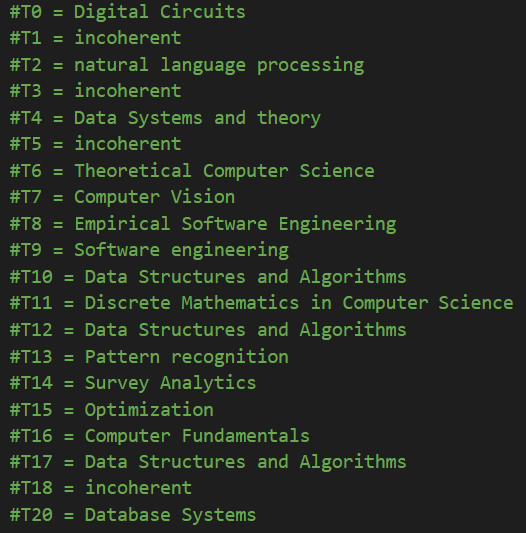
\includegraphics[width=\linewidth]{Figures/before 199Topics.png}
	\caption{20 Topics before 1990}
	\label{fig:ap1990}
\end{figure}

\begin{figure}[ht]\centering
	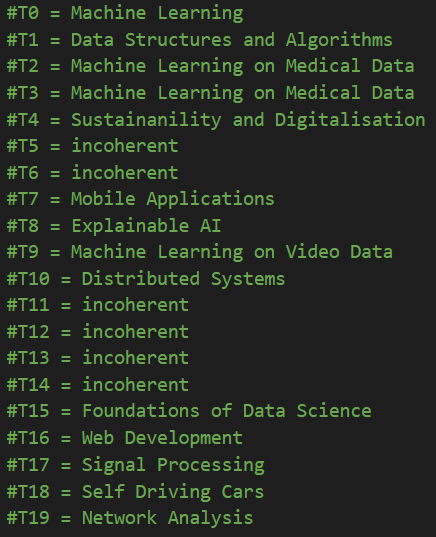
\includegraphics[width=\linewidth]{Figures/before 2010 Topics.png}
	\caption{20 Topics between 1990 and 2010}
	\label{fig:ap2010}
\end{figure}

\begin{figure}[ht]\centering
	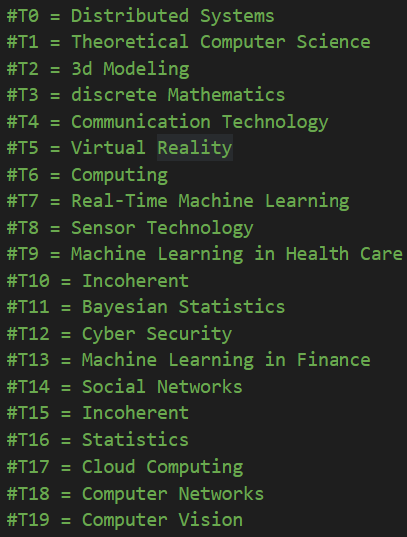
\includegraphics[width=\linewidth]{Figures/After 2010 Topics.png}
	\caption{20 Topics after 2010}
	\label{fig:aptoday}
\end{figure}




%------------------------------------------------


%----------------------------------------------------------------------------------------

\end{document}